% Beamer presentation
\documentclass[11pt,aspectratio=43,ignorenonframetext,t]{beamer}

% Presentation settings
\mode<presentation>{
  \usetheme[framenumber,titleframestart=1]{UoM_alex}
  \usefonttheme{professionalfonts} % using non standard fonts for beamer
  \usefonttheme{serif}
  \usepackage{fontspec}
  \setmainfont[Ligatures=TeX]{Arial}
}

% Handout settings
\mode<article>{
  \usepackage{fullpage}
  \usepackage{fontspec}
  \setmainfont[Ligatures=TeX]{Arial}
  \setlength{\parskip}{1.5\baselineskip} % correct beamer line spacings
  \setlength{\parindent}{0cm}
  \usepackage{enumitem}
  \setlist[itemize]{topsep=0pt}
}

 % Packages
\usepackage{graphicx}
\graphicspath{{./images/png}} % generic graphics path; overridden if necessary
\usepackage{amsmath}
\allowdisplaybreaks[1] % allow eqnarrays to break across pages
\usepackage{amssymb} 
\usepackage[HTML]{xcolor}
\definecolor{uomlinkblue}{HTML}{0071BC}
\usepackage{hyperref}
\hypersetup{
  colorlinks=true,
  linkcolor=uomlinkblue,
  filecolor=uomlinkblue,      
  urlcolor=uomlinkblue,
  pdflang={en-GB},
}
\usepackage[document]{ragged2e} % left aligned text for accessibility
\usepackage{tikz}
\usetikzlibrary{positioning, arrows, arrows.meta}
\usepackage{unicode-math} % unicode maths for accessibility
\usepackage{pdfcomment}   % for alt text for accessibility
\usepackage{rotating}     % allow portrait figures and tables
\usepackage{subfigure}    % allow matrices of figures
\usepackage{float}        % allows H option on floats to force here placement
\usepackage{multirow}     % allows merging of rows in tables
\usepackage{tabularx}     % allows fixed width tables
\usepackage{ctable}       % modifies \hline for use in table
\usepackage{bm}           % allow bold fonts in equations
\usepackage{pgf}          % allow graphics manipulation
\usepackage{etoolbox}
  
% Custom commands
\newcolumntype{Z}{>{\centering\arraybackslash}X}  % tabularx centered columns 

\makeatletter
  \DeclareRobustCommand{\em}
  {
    \@nomath\em
    \if b
      \expandafter\@car\f@series\@nil \normalfont
    \else
      \bfseries
    \fi
  }
\makeatother

\makeatletter
  \preto{\@verbatim}{\topsep=0pt \partopsep=0pt}
\makeatother

\def\checkmark{
  \tikz\fill[scale=0.4](0,.35) -- (.25,0) -- (1,.7) -- (.25,.15) -- cycle;
}

% Counters
\newcounter{example_number} % keep track of the example questions

% Frontmatter
\newcommand{\cmclecture}[1]{
  \title{Combinatorial Mesh Calculus (CMC): Lecture #1}
}
\author{
  Lectured by:
  \href{https://scholar.google.com/citations?user=x4R-snQAAAAJ&hl=en}
  {Dr. Kiprian Berbatov}$^1$\\
  \smallskip
  Lecture Notes Compiled by:
  \href{https://scholar.google.com/citations?user=CoIpITkAAAAJ&hl=en}
  {Muhammad Azeem}$^1$\\
  \smallskip
  Under the supervision of:
  \href{https://scholar.google.co.uk/citations?user=3nWJe5wAAAAJ&hl=en}
  {Prof. Andrey P. Jivkov}$^1$\\
  \smallskip
  {\tiny $^1$Department of Mechanical and Aerospace Engineering,
    The University of Manchester, Oxford Road, Manchester M13 9PL, UK}
}

% Special frames
\newcommand{\cmctitleframe}{
  \titlepage
  \begin{tikzpicture}[remember picture,overlay]
    \node[anchor=south east] at (current page.south east) {
      \href{https://youtube.com/@kipi.berbatov}{
        \includegraphics[width=1.5cm]{youtube-icon.png}
      }
    };
  \end{tikzpicture}
}
\newcommand{\cmcendframe}{
  \begin{figure}
    \centering
    \includegraphics[width=0.85\linewidth]{Thanks.png}
  \end{figure}
}

\cmclecture{6}
\date{22 October 2025}

\begin{document}

%========================= TITLE =========================
\begin{frame}
  \cmctitleframe
\end{frame}

\begin{frame}{Proposition}
\vspace{-0.3cm}
\begin{block}{$\dim \operatorname{Hom}_R(V,W) = (\dim V)(\dim W)$}
Let $R$ be a commutative ring with unity (CRWU). Let $V,W$ be finite free $R$–modules with
\[
\dim V = n,\qquad \dim W = m.
\]
\[
\dim \operatorname{Hom}_R(V,W) \;=\; mn.
\]
\end{block}
\vspace{-0.3cm}
\begin{block}{Proof}
Choose ordered bases $e=(e_1,\dots,e_n)$ of $V$ and $f=(f_1,\dots,f_m)$ of $W$. For each $A\in \operatorname{Hom}_R(V,W)$ write
\[
A(e_j)=\sum_{i=1}^m a_{ij} f_i \quad (1\le j\le n).
\]
\end{block}

\end{frame}

\begin{frame}{Proposition}

\begin{proof}

This identifies $A \longleftrightarrow (a_{ij}) \in M_{m\times n}(R)$. The correspondence
\[
\Phi:\operatorname{Hom}_R(V,W) \simeq M_{m\times n}(R),\quad A\mapsto (a_{ij})
\]
is an $R$–module isomorphism (linearity is entrywise; bijectivity follows by defining a map from any matrix to the unique $A$ with those columns). Hence
\[
\operatorname{Hom}_R(V,W)\cong R^{mn}\quad\Rightarrow\quad \dim \operatorname{Hom}_R(V,W)=mn.\qedhere
\]
\end{proof}
\end{frame}

\begin{frame}{Dual Module}
\begin{block}{Definition.} For a CRWU $R$ and an $R$–module $V$, the \emph{dual module} is
\[
V^* := \operatorname{Hom}_R(V,R) \left[= \{f: V\to R|f\text{ is linear}\}\right].
\]
\end{block}
\begin{block}{Example}
\begin{align*}
(R^2)^*=&\{f:R^2\to R\text{ linear}\,\}\\
=&\{\,f(x_1,x_2)=\lambda_1 x_1+\lambda_2 x_2\mid \lambda_1,\lambda_2\in R\,\}.
\end{align*}

\end{block}
\end{frame}

\begin{frame}{Finite Free Case}

\begin{block}{Remark: Dimension and Basis Dependence}
Let $R$ be a commutative ring with unity (CRWU), and let $V$ be a finite--dimensional (free) $R$--module.
Then
\[
\dim(V^*) = \dim\left(\operatorname{Hom}_R(V, R)\right) = \dim(V).
\]
Indeed, each $R$--linear map $f:V\to R$ is determined uniquely by its values on a basis of $V$.
If $V$ has basis $\{e_1,\dots,e_n\}$, the dual module $V^*$ has the dual basis $\{e^1,\dots,e^n\}$ where $e^i(e_j)=\delta^i_j$; hence both spaces have the same number of basis elements.
\end{block}
\textbf{Summary.}
Although $\dim V = \dim V^*$ and we can identify them under a fixed basis, such identification is artificial - only the double dual $V^{**}$ can be identified with $V$ \emph{canonically}.
\end{frame}

\begin{frame}{Finite Free Case}
\vspace{-0.2cm}
\begin{block}{Interpretation.}
\begin{itemize}
  \item There exists an isomorphism $V\cong V^*$, but it is \emph{not canonical}: it depends on the chosen basis. Different choices of basis lead to different identifications between $V$ and its dual.
  \item Consequently, in general algebraic treatments (over rings that are not fields), we always distinguish $V$ from $V^*$.
  \item In the language of physics and differential geometry:
  \begin{itemize}
    \item Elements of $V$ are \emph{contravariant vectors} — typically represented as column vectors.
    \item Elements of $V^*$ are \emph{covariant vectors} — typically represented as row vectors or linear functionals acting on $V$.
  \end{itemize}
  \item Thus, $V$ and $V^*$ play dual but complementary roles: one represents directions, the other represents measurements (functionals) on those directions.
\end{itemize}
\end{block}

\end{frame}

\begin{frame}{Dual Basis}
\begin{block}{Kronecker Delta}
    Let $V$ be finite free with ordered basis $e=(e_1,\dots,e_n)$. The \emph{dual basis} $e^*=(e^1,\dots,e^n)$ is the family of linear forms $e^i:V\to R$ defined by
\[
e^i(e_j)=\delta^i_j\quad (1\le i,j\le n),
\]
where the \emph{Kronecker delta} is
\[
\delta^i_j=
\begin{cases}
1, & i=j,\\
0, & i\ne j.
\end{cases}
\]
\end{block}

\textbf{Example (standard $\mathbb{R}^2$).} With $e_1=(1,0)$, $e_2=(0,1)$, the dual basis is given by projections
\[
e^1(x_1,x_2)=x_1,\qquad e^2(x_1,x_2)=x_2.
\]
\end{frame}

\begin{frame}{Reconstruction via Dual Basis}
\vspace{-0.2cm}
\begin{block}{Proposition}
Let $V$ be finite free, $e=(e_1,\dots,e_n)$ a basis and $e^*=(e^1,\dots,e^n)$ its dual. Then for every $v\in V$,
\[
v=\sum_{i=1}^n e^i(v)\, e_i.
\]
\end{block}
\vspace{-0.2cm}
\begin{proof}
Write $v=\sum_{j=1}^n \lambda_j e_j$. Apply $e^i$:
\[
e^i(v)=\sum_{j=1}^n \lambda_j e^i(e_j)=\sum_{j=1}^n \lambda_j \delta^i_j=\lambda_i.
\]
Hence $\sum_i e^i(v)e_i=\sum_i \lambda_i e_i=v$.
\end{proof}

\end{frame}

\begin{frame}{Standard \& Nonstandard Basis in $\mathbb{R}^2$}
\begin{block}{Example (standard $\mathbb{R}^2$).} For $v=(v_1,v_2)$ and $e=(e_1,e_2)$ standard,
\[
v=e^1(v)e_1+e^2(v)e_2 = v_1(1,0)+v_2(0,1)=(v_1,v_2).
\]
\end{block}
\begin{block}{Example (nonstandard $\mathbb{R}^2$).}
    Let $e_1=(1,2)$, $e_2=(4,1)$. Seek $e^1,e^2\in (\mathbb{R}^2)^*$ such that
\[
e^1(e_1)=1,\ e^1(e_2)=0,\qquad e^2(e_1)=0,\ e^2(e_2)=1.
\]
\end{block}
\end{frame}

\begin{frame}{Example}
    \begin{block}{}
        \textbf{Solve for $e^1$.} Write $e^1(x_1,x_2)=\lambda_1 x_1+\lambda_2 x_2$. Then
\[
\lambda_1+2\lambda_2=1,\qquad 4\lambda_1+\lambda_2=0.
\]
From the second, $\lambda_2=-4\lambda_1$. Substitute in the first:
\[
\lambda_1-8\lambda_1=1 \Rightarrow -7\lambda_1=1 \Rightarrow \lambda_1=-\frac{1}{7},\quad \lambda_2=\frac{4}{7}.
\]
Thus $e^1(x_1,x_2)=-\frac{1}{7}x_1+\frac{4}{7}x_2$.

\textbf{Solve for $e^2$.} Let $e^2(x_1,x_2)=\mu_1 x_1+\mu_2 x_2$. Then
\[
\mu_1+2\mu_2=0,\qquad 4\mu_1+\mu_2=1.
\]
\end{block}
\end{frame}
\begin{frame}{Example}
\begin{block}{}
    From the first, $\mu_1=-2\mu_2$. Substitute:
\[
-8\mu_2+\mu_2=1 \Rightarrow -7\mu_2=1 \Rightarrow \mu_2=-\frac{1}{7},\quad \mu_1=\frac{2}{7}.
\]
Thus $e^2(x_1,x_2)=\frac{2}{7}x_1-\frac{1}{7}x_2$.\\

\textbf{Check.} One verifies $e^i(e_j)=\delta^i_j$ and the reconstruction
\[
v = e^1(v)\,e_1 + e^2(v)\,e_2 \quad \text{for all } v\in \mathbb{R}^2.
\]
    \end{block}

\end{frame}

\begin{frame}{Matrix View}
\vspace{-0.2cm}
\begin{block}{Dual Rows are the Inverse Matrix}
    Let $E$ be the $2\times 2$ matrix with columns $e_1,e_2$:
\[
E=
\begin{bmatrix}
1 & 4\\
2 & 1
\end{bmatrix},\qquad \det E = 1\cdot 1 - 4\cdot 2 = -7\neq 0.
\]
Then
\[
E^{-1}=\frac{1}{-7}
\begin{bmatrix}
1 & -4\\
-2 & 1
\end{bmatrix}
=
\begin{bmatrix}
-\tfrac{1}{7} & \tfrac{4}{7}\\[2pt]
\tfrac{2}{7} & -\tfrac{1}{7}
\end{bmatrix}.
\]
\end{block}
\vspace{-0.2cm}
\textbf{Observation.} The rows of $E^{-1}$ are exactly the coefficient vectors of $e^1$ and $e^2$:
\[
e^1(x_1,x_2)=\bigl[-\tfrac{1}{7}\ \ \tfrac{4}{7}\bigr]\!\begin{bmatrix}x_1\\ x_2\end{bmatrix},\quad
e^2(x_1,x_2)=\bigl[\tfrac{2}{7}\ \ -\tfrac{1}{7}\bigr]\!\begin{bmatrix}x_1\\ x_2\end{bmatrix}.
\]
Thus $(e^1,e^2)$ corresponds to $E^{-1}$ and $(\cdot)$-coordinates satisfy $v^e=E^{-1} v^{\text{std}}$.
\end{frame}

\begin{frame}{Definition}
\begin{block}{Dual Map}
Let $V,W$ be $R$–modules and $\phi\in\operatorname{Hom}_R(V,W)$. The \emph{dual map}
\[
\phi^*:W^*\longrightarrow V^*,\qquad \phi^*(g):=g\circ \phi
\]
is $R$–linear. In evaluation form, for $g\in W^*$ and $v\in V$,
\[
(\phi^* g)(v) = g\left(\phi(v)\right).
\]
\end{block}


\begin{center}
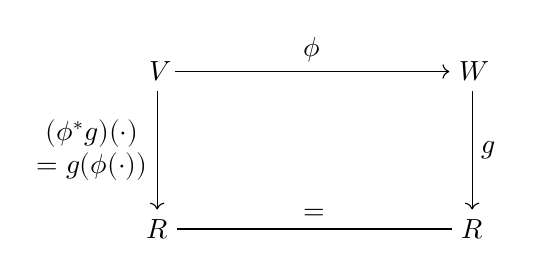
\begin{tikzpicture}
    % Define nodes
    \node (V) at (0,0) {$V$};
    \node (W) at (4,0) {$W$};
    \node (R1) at (0,-2) {$R$};
    \node (R2) at (4,-2) {$R$};

    % Draw arrows
    \draw[->] (V) -- node[above] {$\phi$} (W);
    \draw[->] (V) -- node[left,align=center] {$(\phi^* g)(\cdot)$\\$=g(\phi(\cdot))$} (R1);
    \draw[->] (W) -- node[right] {$g$} (R2);
    \draw (R1) -- node[above] {$=$} (R2);
\end{tikzpicture}
\end{center}
\end{frame}

\begin{frame}{Corollary: Coordinates via Dual Basis}
Let $R$ be a CRWU, $V,W$ finite free $R$–modules with ordered bases
\[
e=(e_1,\dots,e_n)\text{ of }V,\qquad f=(f_1,\dots,f_m)\text{ of }W,
\]
and dual bases $e^*=(e^1,\dots,e^n)$, $f^*=(f^1,\dots,f^m)$. For $\phi\in\operatorname{Hom}_R(V,W)$ and each $j$,
\[
\phi(e_j)=\sum_{i=1}^m f^i(\phi(e_j))\, f_i.
\]
Hence the matrix of $\phi$ w.r.t.\ $(e,f)$ is
\[
(\phi)_e^f=\big\{f^i(\phi(e_j))\big\}_{1\le j\le n}^{1\le i\le m}\in M_{m\times n}(R).
\]
\vspace{-0.2cm}
\begin{proof}
By definition of the dual basis, any $w\in W$ decomposes as $w=\sum_i f^i(w)f_i$. Apply this to $w=\phi(e_j)$.
\end{proof}
\end{frame}





\begin{frame}{Proposition}
\vspace{-0.2cm}
\begin{block}{Matrix of $\phi^*$ is the Transpose of $(\phi)_e^f$}
    Let $V,W$ be finite free, $e=(e_1,\dots,e_n)$, $f=(f_1,\dots,f_m)$ with dual bases $e^*=(e^1,\dots,e^n)$, $f^*=(f^1,\dots,f^m)$. For $\phi\in\operatorname{Hom}_R(V,W)$,
\[
(\phi^*)_{f^*}^{e^*} = \left((\phi)_e^f\right)^{\!T}.
\]
\end{block}
\vspace{-0.2cm}

\begin{block}{Proof}
Write $\phi(e_j)=\sum_{i=1}^m a_{ij} f_i$; thus $(\phi)_e^f=(a_{ij})$. We compute the coordinates of $\phi^*(f^i)\in V^*$ in the basis $e^*$:
\[
\phi^*(f^i)=f^i\circ \phi \in V^*,
\]
so for each $j$, $e^j\left(\phi^*(f^i)\right) = \left(\phi^*(f^i)\right)(e_j) = f^i(\phi(e_j)).$
But $f^i(\phi(e_j))=a_{ij}$ by the very definition of the coefficients $a_{ij}$.
\end{block}

\end{frame}

\begin{frame}{Proof}
\vspace{-0.3cm}
\begin{block}{}
 Hence the $j$-th coordinate of $\phi^*(f^i)$ w.r.t.\ $e^*$ equals $a_{ij}$. Therefore, the matrix with columns $\big[\phi^*(f^1)\big]_{e^*},\dots,\big[\phi^*(f^m)\big]_{e^*}$ is $(a_{ij})$ with indices swapped, i.e.
\[
(\phi^*)_{f^*}^{e^*}=(a_{ji})=\left((\phi)_e^f\right)^{\!T}.
\]
\end{block}
\vspace{-0.7cm}
\begin{center}
\begin{tikzpicture}
    % Define nodes
    \node (V) at (0,2) {$V$};
    \node (W) at (4,2) {$W$};
    \node (Wstar) at (0,0) {$W^*$};
    \node (Rm) at (4,0) {$R^m$};
    \node (Rn) at (0,-2) {$R^n$};

    % Draw arrows
    \draw[->] (V) -- node[above] {$\phi$} (W);
    \draw[->] (Wstar) -- node[left] {$\phi^*$} (V);
    \draw[->,dashed] (Wstar) -- node[above] {$(\cdot)^{f^*}$} (Rm);
    \draw[->,dashed] (Rm) -- node[right] {$((\phi)_e^f)^{T}(\cdot)$} (W);
    \draw[->,dashed] (Rn) -- node[left] {$(\cdot)_{e^*}^{-1}$} (Wstar);
\end{tikzpicture}
\end{center}

\end{frame}


\begin{frame}{Dual Reverses Composition}
\textbf{Proposition.} Let $U,V,W$ be $R$–modules, $\phi\in\operatorname{Hom}_R(U,V)$, $\psi\in\operatorname{Hom}_R(V,W)$. Then
\[
(\psi\circ \phi)^*=\phi^*\circ \psi^* : W^*\to U^*.
\]

\begin{proof}
For $g\in W^*$ and $u\in U$,
\begin{align*}
    \left((\psi\circ \phi)^* g\right)(u)=&g\left((\psi\circ \phi)(u)\right)=g\left(\psi(\phi(u))\right)=(\psi^* g)\left(\phi(u)\right)\\
=&(\phi^*(\psi^* g))(u).
\end{align*}
Since both sides define the same functional on every $u$, we have equality of maps $W^*\to U^*$.
\end{proof}

\end{frame}

\begin{frame}{Dual Reverses Composition}
\begin{block}{}
\begin{enumerate}
    \item The sequence of maps on the vector spaces runs in the forward direction:
    $$ U \xrightarrow{\phi} V \xrightarrow{\psi} W $$
    \item The sequence of the dual maps runs in the reverse direction:
    $$ W^* \xleftarrow{\psi^*} V^* \xleftarrow{\phi^*} U^* $$
\end{enumerate}
The dual map $\phi^*$ is defined by $(\phi^* f)(u) = f(\phi(u))$, where $f \in V^*$ and $u \in U$. The composition rule for duals also reverses the order: $(\psi \circ \phi)^* = \phi^* \circ \psi^*$.


\end{block}

\end{frame}

\begin{frame}{Canonical Evaluation Map $\iota:V\to V^{**}$}
\textbf{Definition.} For any $R$–module $V$, define the \emph{evaluation} (canonical) map
\[
\iota:V\longrightarrow V^{**}=\operatorname{Hom}_R(V^*,R),\qquad
\iota(v)(f):=f(v)\quad (f\in V^*).
\]

\begin{center}
\begin{tikzpicture}[>=Latex, node distance=3cm, auto] % Setting global styles

    % 1. Define Nodes: V, V**, and R
    \node (V) at (0, 0) {$V$};
    \node (Vss) [right=of V] {$V^{**}$}; % V** is 3cm to the right of V
    \node (R) [below=of Vss] {$R$}; % R is 3cm directly below V**

    % 2. Draw Forward Map (V -> V**) - Canonical Isomorphism
    \draw[->] (V) -- (Vss) node[midway, above] {$\iota$};

    % 3. Draw Diagonal Map (V -> R) - Evaluation by f
    % Note: f is a functional, f \in V^*
    \draw[->] (V) -- (R) node[midway, below left] {$f$};

    % 4. Draw Downward Map (V** -> R) - Evaluation Map
    % The arrow is dashed as it often represents a construction or evaluation process.
    \draw[->, dashed] (Vss) -- (R) node[midway, right] {$(\cdot)(f)$};
\end{tikzpicture}
\end{center}

\end{frame}

\begin{frame}{Proposition}

\begin{block}{Finite Free Case} If $V$ is finite free, then $\iota$ is an isomorphism; we write $V \simeq V^{**}$ \emph{canonically}.

\end{block}

\begin{proof}
Fix a basis $e=(e_1,\dots,e_n)$ with dual $e^*=(e^1,\dots,e^n)$. Then $\iota(e_j)$ is the functional on $V^*$ sending $f$ to $f(e_j)$. In the dual basis, $\iota(e_j)$ corresponds to the coordinate row $(e^1(e_j),\dots,e^n(e_j))=(0,\dots,1,\dots,0)$, hence $\iota$ sends a basis to a basis and is therefore an isomorphism. Basis-independence: if we change basis by an invertible matrix $E$, the dual basis changes by $E^{-1\,T}$, and the resulting matrix of $\iota$ remains the identity; thus $\iota$ is canonical.
\end{proof}
\end{frame}

\begin{frame}{Naturality with Respect to Double Dual}
\vspace{-0.5cm}
\begin{block}{}
Let $V,W$ be finite free, and $\phi\in\operatorname{Hom}_R(V,W)$. The double dual map $\phi^{**}:V^{**}\to W^{**}$ is defined by
\[
\phi^{**}(\Lambda):= \Lambda\circ \phi^*,\qquad (\Lambda\in V^{**}).
\]
Then the square commutes:
\vspace{-0.7cm}
\begin{center}
\begin{tikzpicture}[>=Latex, node distance=3cm, auto]

    % 1. Define Nodes: V, W, V**, and W**
    \node (V) {$V$};
    \node (W) [right=of V] {$W$};
    \node (Vss) [below=of V] {$V^{**}$};
    \node (Wss) [below=of W] {$W^{**}$};

    % 2. Draw Top Arrow (V -> W)
    \draw[->] (V) -- (W) node[midway, above] {$\phi$};

    % 3. Draw Left Arrow (V -> V**)
    \draw[->] (V) -- (Vss) node[midway, left] {$\iota_V$};

    % 4. Draw Right Arrow (W -> W**)
    \draw[->] (W) -- (Wss) node[midway, right] {$\iota_W$};

    % 5. Draw Bottom Arrow (V** -> W**)
    \draw[->] (Vss) -- (Wss) node[midway, below] {$\phi^{**}$};
\end{tikzpicture}
\end{center}

\end{block}
\end{frame}

\begin{frame}{Proof}

\begin{proof}
For $v\in V$ and $g\in W^*$,
\begin{align*}
\left(\phi^{**}\circ \iota_V\right)(v)(g)=& \iota_V(v)(\phi^* g) = (\phi^* g)(v)=g(\phi(v))\\
=& \iota_W(\phi(v))(g)\\
=& \left(\iota_W\circ \phi\right)(v)(g).
\end{align*}
Thus $\phi^{**}\circ \iota_V=\iota_W\circ \phi$.
\end{proof}

\end{frame}

\begin{frame}{Bilinear Maps and Currying}
\begin{block}{Definition.} Let $U,V,W$ be $R$–modules. A map $\Phi:U\times V\to W$ is \emph{bilinear} if
\[
\Phi(u_1+u_2,v)=\Phi(u_1,v)+\Phi(u_2,v),\quad
\Phi(\lambda u,v)=\lambda \Phi(u,v),
\]
\[
\Phi(u,v_1+v_2)=\Phi(u,v_1)+\Phi(u,v_2),\quad
\Phi(u,\lambda v)=\lambda \Phi(u,v).
\]
Equivalently, the \emph{curried} map $\widetilde{\Phi}:U\to \operatorname{Hom}_R(V,W)$, $\widetilde{\Phi}(u)(v)=\Phi(u,v)$, is $R$–linear:
\[
\Phi\in \mathcal{L}(U,V;W) \iff \widetilde{\Phi}\in \operatorname{Hom}_R\left(U,\operatorname{Hom}_R(V,W)\right).
\]

\end{block}

\end{frame}

\begin{frame}{Examples}
 \begin{itemize}
\item Dot product (over a CRWU contained in $\mathbb{R}$): $\langle x,y\rangle=\sum_{i=1}^n x_i y_i:\ R^n\times R^n\to R$ is bilinear.
\item Evaluation: $\mathrm{eval}:V\times V^*\to R$, $\mathrm{eval}(v,f)=f(v)$ is bilinear since it is linear in each entry.
\end{itemize}

\begin{center}
\begin{tikzpicture}[>=Latex, node distance=4cm, auto] % Increased node distance for better spacing of Hom-space

    % 1. Define Nodes
    \node (UV) {$U \times V$};
    \node (W) [right=of UV] {$W$};
    \node (U) [below=of UV] {$U$};
    % Note: Hom_R is larger, so we align its bottom position with U
    \node (Hom) [below right=of W, yshift=1cm] {$\operatorname{Hom}_R(V, W)$}; % Adjusted for vertical alignment
    \node at (Hom.north) [yshift=-1cm] {}; % Helper node for alignment

    % 2. Draw Arrows
    % Top: U x V -> W
    \draw[->] (UV) -- (W) node[midway, above] {$\Phi$};

    % Left: U x V -> U (Curry map)
    \draw[->, dashed] (UV) -- (U) node[midway, left] {$\text{curry}$};

    % Bottom: U -> Hom_R(V, W)
    \draw[->] (U) -- (Hom) node[midway, below] {$\widetilde{\Phi}$};

    % Right/Up: Hom_R(V, W) -> W (Evaluation map)
    % We need to manually adjust the start and end points of the evaluation arrow
    \draw[->, dashed] (Hom.north) -- (W.south) node[midway, right] {$\mathrm{ev}$};

\end{tikzpicture}
\end{center}
\end{frame}

\begin{frame}{Thanks}
  \cmcendframe
\end{frame}

\end{document}
